\Chapter{Jellemzők kinyerése}

% TODO: Összeszedni a jellemzően használt feature-öket. (Az előző fejezetből át lehet emelni az ide vonatkozó részeket.)

% TODO: Meg kellene nézni, hogy ebből mit és hogy lehetne implementálni \cite{trier1996feature} : http://citeseerx.ist.psu.edu/viewdoc/download?doi=10.1.1.51.7439&rep=rep1&type=pdf

% TODO: Átnézni, és kivenni a megfelelő részeket \cite{liu2008handwritten}: https://hal.inria.fr/file/index/docid/120408/filename/liama2.pdf

% TODO: \cite{liu2006high} https://hal.inria.fr/file/index/docid/120419/filename/liama4.pdf

A gépi tanulásban, a minta felismerésében és a képfeldolgozásban a funkciókivonás a mért adatok kezdeti sorozatából indul ki és nem redundáns szándékú származtatott értékeket (jellemzőket) hoz létre. A jellemzők elősegítik a későbbi tanulási és általánosítási lépéseket és egyes esetekben a jobb emberi értelmezést. A funkciókivonás\cite{features27:online} összefügg a dimenzionalitás csökkentésével.

Ha egy algoritmushoz tartozó bemeneti adat túl nagy ahhoz, hogy feldolgozni lehessen, mert gyaníthatóan redundáns (pl. a képpontként ismétlődése a megjelenített képeken), akkor átalakítható egy csökkentett készletté (funkcióvektorként is nevezik). A kezdeti funkciók egy részhalmazának meghatározása a funkciókiválasztásnak nevezik. A kiválasztott funkciók várhatóan tartalmazzák a bemeneti adatok releváns adatait, így a kívánt feladat a teljes kezdeti adat helyett a csökkentett ábrázolás használatával végezhető el.

\section{Dimenzió redukció}
\begin{itemize}
\item PCA: A dimenziócsökkentés\cite{wang2003feature} fő lineáris technikája a főkomponens elemzés, az adatok lineáris leképezését végzi egy alsó dimenziós térben. A főkomponens-elemzés (PCA) az osztályozási problémák dimenzió csökkentési technikájaként használható. A dimenziócsökkentés fő lineáris technikája, főkomponens elemzés, az adatok lineáris leképezését végzi egy alsó dimenziós térben.

A gyakorlatban az adatok kovariancia mátrixát állítják össze és a mátrixban lévő sajátvektorokat kiszámítják. A legnagyobb sajátértékeknek megfelelő sajátvektorok a főkomponensek, amelyek felhasználhatók az eredeti adatok nagy részének rekonstruálására.

Ha létezik egy $A$ nevű négyzetes mátrix, egy skalár $\lambda$ és egy nem nulla vektor $v$, akkor $\lambda$ az sajátérték és a $v$ a sajátvektor, ha a következő egyenlet teljesül:

$$
Av = \lambda v
$$

\item Kernel PCA: A fő komponenselemzés nemlineáris módon használható az úgynevezett kernel trükkel. Az így kapott technika képes nemlineáris leképezések létrehozására, amelyek maximalizálják az adatokban a varianciát.

Példa egy lineárisan nem szeparálható adathalmazra \aref{fig:kernel_pca_input} ábrán látható:

\begin{figure}[h]
\centering
\captionsetup{justification=centering}
\begin{tabular}{ c c }
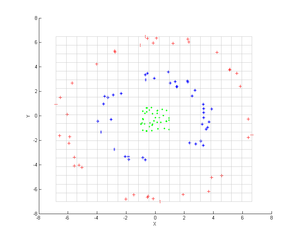
\includegraphics[scale=0.8]{images/kernel_pca_input} & 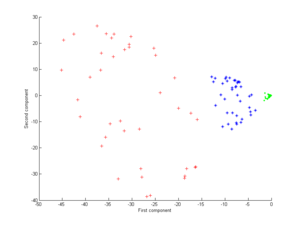
\includegraphics[scale=0.8]{images/kernel_pca_output}
\end{tabular}
\caption[caption]{Bementi pontok kernel PCA transzformáció után
\hspace{\textwidth}Forrás:\url{https://en.wikipedia.org/wiki/Kernel_principal_component_analysis}}
\label{fig:kernel_pca_input}
\end{figure}

\Aref{fig:kernel_pca_input} ábra bal oldali képen az adatok lineárisan nem szeparálhatók. A kernel PCA transzformáció során olyan teret képezünk le (\aref{fig:kernel_pca_input} ábra jobb oldali kép), ahol az adatok lineáris leképezés lehetséges.

A kernel meghatározása:
$$
k({\boldsymbol  {x}},{\boldsymbol  {y}})=({\boldsymbol  {x}}^{{\mathrm  {T}}}{\boldsymbol  {y}}+1)^{2}
$$

Lehetőségünk van különböző kernelek definiálására, felsorolok néhány példát: \textit{Gauss kernel:} $e^{{\frac  {-||{\boldsymbol  {x}}-{\boldsymbol  {y}}||^{2}}{2\sigma ^{2}}}}$ \textit{, Tangens kernel:} $tanh(({\bf x}\cdot {\bf y})+\theta)$ \textit{, Polinom kernel:} $({\bf x}\cdot {\bf y})^k$

\item LDA\cite{wang2003feature}: A lineáris diszkriminancia-analízis (LDA) a Fisher lineáris diszkriminánsának, a statisztikában, a minta felismerésében és a gépi tanulásban használt módszer, amely olyan objektumok lineáris kombinációját találja, amely két vagy több objektum- vagy eseményosztályt jellemez vagy elválaszt.
\item Autoencoder: Az "autoencoding" egy olyan adattömörítési algoritmus, ahol a tömörítési és dekompressziós függvények:
\begin{enumerate}
\item adat-specifikusak: Az autoencoderek adatspecifikusak, ami azt jelenti, hogy csak azokat az adatokat tudják tömöríteni, amelyekkel betanították.
\item veszteségesek: Az autoencoderek veszteségesek, ami azt jelenti, hogy a dekompresszált kimenetek az eredeti bemenetekhez képest romlanak.
\item automatikusan tanul: Tanulnak a példákból, nem pedig ember által előtervezettek.
\end{enumerate}
Minden olyan környezetben, ahol az "autoencodert" használják, a kompressziós és dekompressziós funkciókat neurális hálózatokkal valósítják meg.

Ma az autoencoderek két érdekes gyakorlati alkalmazása az adatok zajszűrése és az adatok dimenziócsökkentése. Megfelelő dimenzionalitással az autoencoderek jobban teljesítenek mint a PCA vagy egyéb alapvető technikák.

Az autoencoder implementálása a \textit{keras} könyvtár, a  \textit{layers} és \textit{models} modulok használatával:
\begin{python}

input_img = Input(shape=(784,)) # A bemeneti adat
encoded = Dense(32, activation='relu')(input_img) # kodolt adat
decoded = Dense(784, activation='sigmoid')(encoded) # dekodolt adat
# Az autoencoder, encoder, decoder modell
autoencoder = Model(input_img, decoded)
encoder = Model(input_img, encoded)
encoded_input = Input(shape=(32,))
decoder_layer = autoencoder.layers[-1] # Autoencoder utolsó rétege
decoder = Model(encoded_input, decoder_layer(encoded_input))
\end{python}
\begin{python}
autoencoder.compile(optimizer='adadelta', loss='binary_crossentropy')
\end{python}
A fordítás után következhet a tanítás
\begin{python}
autoencoder.fit(x_train, x_train,	# A tanito es a cel
                epochs=50,		# adatok megegyeznek
                batch_size=256,
                shuffle=True,
                validation_data=(x_test, x_test))
\end{python}
\end{itemize}

A neurális hálózat szerkezete \aref{fig:deep_autoencoder} ábrán látható:
\begin{figure}[h]
\centering
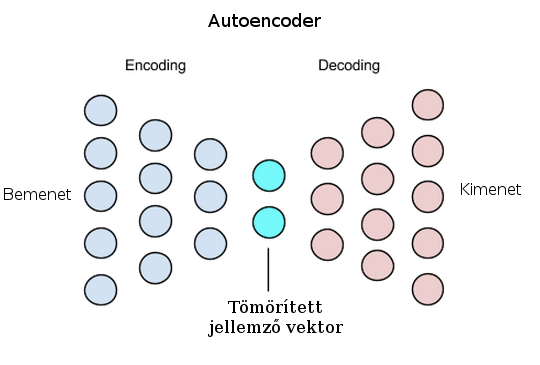
\includegraphics[scale=0.6]{images/deep_autoencoder}
\caption{Autoencoder}
\label{fig:deep_autoencoder}
\end{figure}

A neurális hálózatunk szimmetrikus. A középső rejtett rétegen az adatunk tömörített változatát találhatjuk. Számunkra nem a kimenet az érdekes, hiszen az csak egy másolata a bementi rétegnek. A rejtett rétegek súlyai fontosak számunkra. Az előállított súlyokkal képesek vagyunk az adatok dimenzió csökkentésére. A kép egy tömörített változata elősegíti a gyorsabb feldolgozást.

\section{Alacsony szintű jellemzők}
Az alacsony szintű jellemző\cite{features27:online}, amelyek a kép tartalmát leíró technikák, egy teljes kép szintjén, nem pedig annak különböző területein. Az egyik legfontosabb folyamat, amellyel találkozunk, az úgynevezett éldetektálás.
\begin{itemize}
\item Éldetektálás: Az éldetektálás számos matematikai módszert foglal magában, amelyek olyan pontok azonosítását célozzák meg egy digitális képen, amelyeknél a kép fényereje élesen megváltozik vagy formálisan megszakad. Azok a pontok, amelyeknél a kép fényereje élesen változik, tipikusan íves szegmensek csoportjába sorolják.
Kép fényerejének hirtelen változásainak okai lehetnek:
\begin{enumerate}
\item Hirtelen mélységi változás
\item Felület normálisának változása
\item Megvilágítás változása: árnyékok, világítás változás
\item Visszaverődésben változás: felület tulajdonság
\end{enumerate}
\item Sarokérzékelés: A sarokérzékelés egy olyan megközelítés, amelyet a számítógépeslátásnál használnak bizonyos jellemzők kivonására és a kép tartalmának kivonására.
A sarok két él metszéspontjaként definiálható. A sarok olyan pontként is definiálható, amelynél a pont egy helyi szomszédságában két domináns és különböző él irány található.
Harris és Stephens sarokdetektáló algoritmus rendkivül gyors. A szürkeárnyalatos kétdimenziós képeknél alkalmazhatjuk. Adjuk meg ezt a képet $I$ segítségével. Vegyünk egy képpontot a $(u, v)$ területen és mozgassuk azt $(x, y)$. A két pont közötti négyzetes különbség (SSD) súlyozott összege, $S$, az alábbiak szerint adható meg:

$$
S(x,y)=\sum_{u}\sum_{v}w(u,v)(I(u+x,v+y)-I(u,v))^{2}
$$

A Harris mátrix:

$$
{\displaystyle A=\sum _{u}\sum _{v}w(u,v){\begin{bmatrix}I_{x}(u,v)^{2}&I_{x}(u,v)I_{y}(u,v)\\I_{x}(u,v)I_{y}(u,v)&I_{y}(u,v)^{2}\end{bmatrix}}={\begin{bmatrix}\langle I_{x}^{2}\rangle &\langle I_{x}I_{y}\rangle \\\langle I_{x}I_{y}\rangle &\langle I_{y}^{2}\rangle \end{bmatrix}}}
$$

Ahol:\\
$I_x$: Az adott derivált az x-irányban\\
$I_y$: Az adott derivált az y-irányban\\
$w(x, y)$: Súlyozási függvény (pl. Gaussian)

Egy sarkot az $(x, y)$ vektor minden irányának $S$ változata jellemez. Az $A$ sajátértékének elemzésével ezt a jellemzést a következő módon fejezhetjük ki: $A$-nak két sajátértékkel kell rendelkeznie egy sarok pontra. A sajátértékek nagyságrendje alapján az alábbi következtetésekre lehet következtetni:
\begin{enumerate}
\item Ha $\lambda _{1}\approx 0$ és $\lambda_2 \approx 0$ akkor az $(x,y)$ képpontnak nincs sarok jellemzője.
\item Ha $\lambda_1 \approx 0$ és $\lambda _{2}$ egy nagy pozítiv szám, akkor sarok található.
\item Ha $\lambda_1$ és $\lambda_2$ nagy pozítiv szám, akkor sarok detektálható.
\end{enumerate}
\item Méret-invariáns jellemző transzformáció (SIFT): A transzformáció a számítógéplátásban használt algoritmus, amely helyi jellemzők felderítésére és leírására használják. A kulcspontokat az objektumokon először egy kép készletből vonják ki és tárolják egy adatbázisban. Egy objektumot felismerünk egy új képen azáltal, hogy az egyes képeket az új képből az adatbázisba hasonlítjuk össze és megtaláljuk a megfelelő jellemzőket, amelyek euklideszi távolságukon alapulnak. \Aref{fig:sift} ábrán látható egy példa.
\begin{figure}[h]
\centering
\captionsetup{justification=centering}
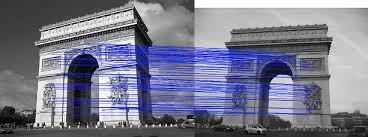
\includegraphics[scale=1.0]{images/sift}
\caption{A jellemzők felderítése elforgatott képen \hspace{\textwidth}Forrás:\url{http://www.ismailsirma.com/visualsfm-3d-construction-of-images}}
\label{fig:sift}
\end{figure}
\end{itemize}

\section{Irány szerinti jellemző kinyerés}
Figyelembe véve, hogy a kínai karakterek stroke részei megközelíthetők többféle irányba. A korai munkákban négy irányba (vertikális, horizontális, bal átlós és jobb átlós) bontották fel a karaktereket. A képpontok nyolc irányba történő bontása (\aref{fig:direction8} ábra) négy irány helyett jelentősen javította a felismerési pontosságot. Ez azért van így, mert a stroke két oldalának elválasztása jobban megkülönbözteti a párhuzamos stroke-okat.

\begin{figure}[h]
\centering
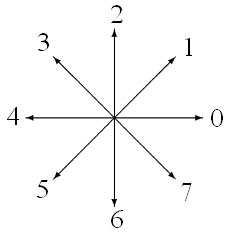
\includegraphics[scale=0.5]{images/direction8}
\caption{8 irányú felbontás}
\label{fig:direction8}
\end{figure}

Az irány funkciók kinyerése\cite{liu2008handwritten} három lépésben valósul meg: kép normalizálása, irány dekompozíció és jellemző mintavételezés. 

A normalizálás szabályozza a karakterek kép méretét, pozícióját és alakját, hogy csökkentse az azonos osztályú képek közötti változatokat.

\subsection{Irány dekompozíció}

Az irány dekompozíció több iránysíkot eredményez, $f_i(x, y), i = 1,. . . , N_d$. Először leírjuk a gradiens dekompozícióra szolgáló eljárásokat 8 irányban, majd kiterjeszük 12 és 16 irányba.

A gradiens irányú jellemző kinyerés a gradiensvektor, amelyet a normalizált képen számolunk ki a Sobel operátorral, ami 8 irányra bontja a komponenseket. A Sobel operátornak két maszkja van, hogy kiszámítsa a gradiens komponensek a két tengelyen. A maszkok \aref{fig:sobel_operator} ábrán látható.

\begin{figure}[h]
\centering
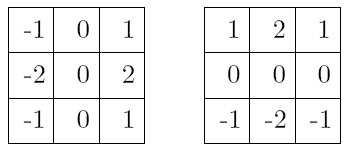
\includegraphics[scale=0.5]{images/sobel_operator}
\caption{Sobel operátor}
\label{fig:sobel_operator}
\end{figure}

Ha egy gradiens irány két standard irány között fekszik, akkor a vektor két komponensre bomlik. Az egyes komponensek hossza a (x, y) képponthoz tartozó megfelelő irány síkhoz van hozzárendelve.

\subsection{Elmosódás és mintavétel}

Mindegyik irány síkot, amelynek méretével megegyezik a normalizált kép azt csökkenteni kell, hogy mérsékelt dimenziójú jellemző értékeket nyerjen. Egy egyszerű módja az, hogy az irány síkot több blokkzónába osztjuk és az egyes zónák teljes vagy átlagos értékét jellemző értékként vesszük.

Az elmosódás végrehajtásakor a térbeli szűrő impulzus-válaszfüggvénye (IRF) egy súlyozott ablakhoz hasonlít, amelyet elmosódási maszknak is neveznek. Az IRF-t gyakran Gaussian függvényként veszik figyelembe:

$$
g(x,y) = \frac{1}{\sqrt{2\pi}\sigma} e^{{(- \frac{x^2 + y^2}{2 \sigma_x^2})}}
$$

A mintavételi tétel szerint a $\sigma_x$ variancia-paraméter a mintavételi frekvenciához kapcsolódik. A Gauss-szűrő sávszélességének az empirikus képlet az alábbi $\sigma_x = \frac{\sqrt{2}t_x}{\pi}$, ahol $t_x$ a mintavételi intervallum.

A kivont jellemzőértékek változók. A transzformáció az változók sűrűségfüggvényét közelebb hozhatja a Gaussian függvényhez. Ez segít a statisztikai osztályozás teljesítményének javításában.

\subsection{Számítási idők}
A jellemző kinyerés CPU időtartama szinte független a normalizációs módszertől. Két részből áll: irány dekompozíció és elmosódás. A három irányú jellemzők átlagos CPU-ideje
\aref{cpu_times} táblázat mutatja. Az elmosódás feldolgozási ideje függ az irányok szűkösségétől (a nulla pixeleket nem veszi figyelembe).

\begin{table}[h]
\centering
\caption{CPU idők}
\label{cpu_times}
\begin{tabular}{|l|l|r|}
\hline
\multicolumn{1}{|c|}{} & direction & blurring \\ \hline
chn                    & 0.121     & 0.439    \\ \hline
nccf                   & 0.458     & 0.752    \\ \hline
grd-g                  & 0.329     & 1.276    \\ \hline
\end{tabular}
\end{table}

\subsection{Korlátozás nélküli minták}
A korlátozás nélküli kézzel készített mintákkal rendelkező képzési osztályozók képesek lesznek javítani a korlátozás nélküli karakterfelismerés pontosságát. A korlátozás nélküli karakterek nagy adatbázisának gyűjtése sürgős feladat lesz a közeljövőben.

Ha a hibaarányt meglehetősen alacsony szintre szeretné csökkenteni (például 2\% -ot az elszigetelt karakterek esetében), egyszerűen csak az aktuális normalizációs és funkciókivonási módszerek használata nem elegendőek. A normalizálás, a funkciókivonás és az osztályozó kialakításának módszereit újra kell gondolni a írásjelek jobb felismerésére. A képzési osztályozók diszkriminatív módon javíthatják a kézírásos és a korlátozás nélküli karakterfelismerés pontosságát.